\documentclass[11pt]{article}

% Packages
\usepackage{graphicx}   % for pictures
\usepackage{amsthm}     % for math
\usepackage{amsmath, mathtools}    %   more math
\usepackage{amsfonts}   %   more math
\usepackage{physics}    % more symbols
\usepackage{circuitikz} % for circuit diagrams
\usepackage{amssymb}    % math symbols
\usepackage{siunitx}    % units
\usepackage{mathrsfs}   % fancy text
\usepackage{color}      % colored letters for notes and reminders
\usepackage{float}      % for image location

%The amsthm package lets you format different types of mathematical ideas nicely. You use it by defining "\newtheorem"s as below:
\newtheorem{problem}{Problem}
\newtheorem{theorem}{Theorem}
\newtheorem*{proposition}{Proposition}
\newtheorem{lemma}[theorem]{Lemma}
\newtheorem{corollary}[theorem]{Corollary}
\theoremstyle{definition}
\newtheorem{defn}[theorem]{Definition}

% Magins

\setlength{\voffset}{0.1in}
\setlength{\paperwidth}{8.5in}
\setlength{\paperheight}{11in}
\setlength{\headheight}{14pt}
\setlength{\headsep}{0.5in}
\setlength{\textheight}{11in}
\setlength{\textheight}{8in}
\setlength{\topmargin}{-0.25in}
\setlength{\textwidth}{7in}
\setlength{\topskip}{0in}
\setlength{\oddsidemargin}{-0.25in}
\setlength{\evensidemargin}{-0.25in}

% For images in this document:
\graphicspath{ {images/} }

% User Defined Commands
\newcommand{\nder}[2]{\frac{d^{#1} #2}{d t^{#1}}}   % The nth derivative wrt t: {n}{x(t)}
\newcommand{\der}[1]{\frac{d #1}{d t}}              % Derivative wrt t: {x(t)}
\newcommand{\infint}{\int_{-\infty}^{\infty}}       % Integral from - infinity to + infinity
\newcommand{\infsum}[1]{\sum_{#1 = -\infty}^{\infty}}% Sum of a variable from - to + infinity
\newcommand{\para}[1]{\left( #1 \right)}            % Instead of writing parenthesis all the time



% Heading:
\usepackage{fancyhdr}
\pagestyle{fancy}
\lhead{Nicholas Pham}
\chead{ES 155}          %   Change the Class!!
\rhead{Homework 2}   %   Change the Problem Set Number!!


% ----- BEGIN DOCUMENT-----
\begin{document}

\textbf{\huge{ES 155 Homework 2}}    %   Change the Class and Problem Set Number!!
\normalsize

\begin{enumerate}
    \item % Problem 1

    In RLC circuit in Figure \ref{fig:RLCcircuit}, $V_s$ is the source voltage, $V_L$ is the voltage on he inductor with inductance $L$, $I_L$ is the current through that inductor, $V_C$ is the voltage across the capacitor with capacitance $C$, and $R$ is the resistance of a resistor in parallel with the capacitor.

    \begin{figure}[h]
    	\centering
    	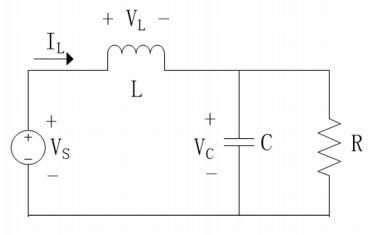
\includegraphics[width = 0.4 \textwidth]{ES155P2_1_RLCcircuit.png}
    	\caption{RLC circuit}
    	\label{fig:RLCcircuit}
    \end{figure}

    The input to the system is the source voltage $V_S$, which can be any time-varying signal.

    \begin{enumerate}
    	\item % Part a
    	Given control input $u(t) = V_S(t)$ with output $y(t) = V_C(t)$, define the state $x(t)$ as

    	\begin{align}
    		x(t) &= \begin{bmatrix} x_1(t) \\ x_2(t) \end{bmatrix} = \begin{bmatrix} V_C(t) \\ I_L(t) \end{bmatrix}
    	\end{align}

    	This gives 

    	\begin{align}
    		\dot{x}(t) &= \begin{bmatrix} \dot{x_1}(t) \\ \dot{x_2}(t) \end{bmatrix} = \begin{bmatrix} \dot{V_C}(t) \\ \dot{I_L}(t) \end{bmatrix}
    	\end{align}

        Substituting the capacitor and inductor equations,

        \begin{align}
            \dot{x}(t) &=  \begin{bmatrix} \dot{V_C}(t) \\ \dot{I_L}(t) \end{bmatrix} = \begin{bmatrix} \frac{1}{C} I_C(t) \\ \frac{1}{L} V_L(t) \end{bmatrix} 
        \end{align}

        Using Kirchoff's Voltage and Current Laws this can be written

        \begin{align}
            \dot{x}(t) &=  \begin{bmatrix} \frac{1}{C} (I_L - I_R) \\ \frac{1}{L} (V_S - V_C) \end{bmatrix} = \begin{bmatrix} \frac{1}{C} (I_L - \frac{V_R(t)}{R}) \\ \frac{1}{L} (V_S - V_C) \end{bmatrix} = \begin{bmatrix} \frac{1}{C} (I_L - \frac{V_C}{R}) \\ \frac{1}{L} (V_S - V_C) \end{bmatrix}
        \end{align}

        Now in terms of $x(t)$ we can write the state space model:

        \begin{align}
            \dot{x}(t) &=  \begin{bmatrix} \dot{x_1}(t) \\ \dot{x_2}(t) \end{bmatrix} = \begin{bmatrix} \frac{1}{C} (x_2(t) - \frac{x_1(t)}{R}) \\ \frac{1}{L} (u(t)- x_1(t)) \end{bmatrix} \\
            y(t) &= x_1(t)
        \end{align}

        In matrix form, $\dot{x}(t) = A x(t) + B u(t)$ and $y(t) = C x(t) + D u(t)$:

        \begin{align}
            \dot{x}(t) &=  \begin{bmatrix} -\frac{1}{RC} & \frac{1}{C} \\ -\frac{1}{L} & 0 \end{bmatrix} \begin{bmatrix} x_1(t) \\ x_2(t) \end{bmatrix} + \begin{bmatrix} 0 \\ \frac{1}{L} u(t) \end{bmatrix} \\
            y(t) &= \begin{bmatrix} 1 & 0 \end{bmatrix} \begin{bmatrix} x_1(t) \\ x_2(t) \end{bmatrix} + \begin{bmatrix} 0 \end{bmatrix} u(t)
        \end{align}


    	\item % Part b
    	Let $R = 1\Omega$, $L = 0.1H$, and $C = 0.2F$.  Figure \ref{fig:phaseportrait} shows the phase portrait for the system.  See attached MATLAB code.  Note: this phase portrait represents the autonomous system with no control input $u(t) = V_S(t)$.

    	\begin{figure}[h]
    		\centering
    		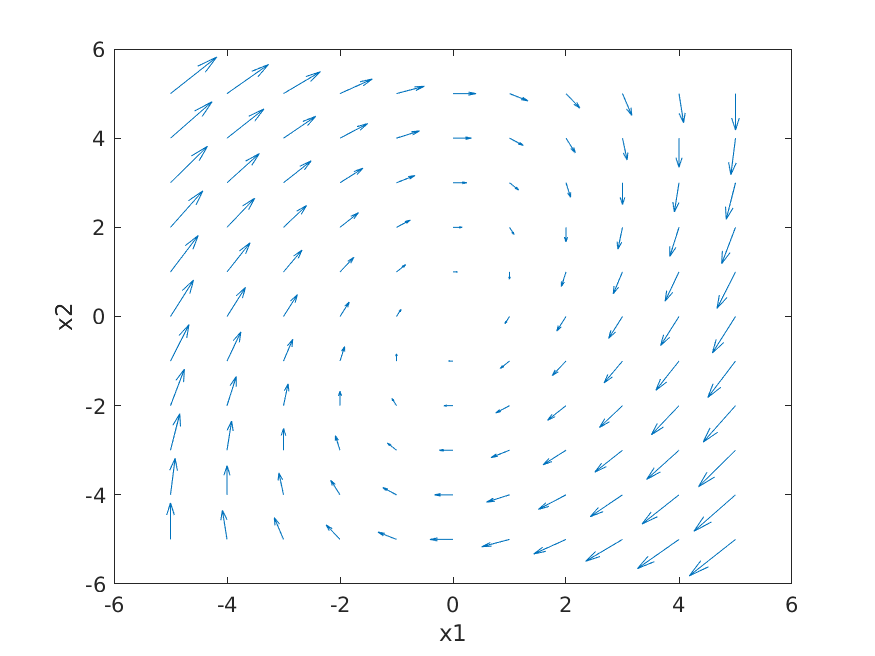
\includegraphics[width = 0.6 \textwidth]{ES155P2_1b_phaseportrait.png}
    		\caption{Phase Portrait describing RLC circuit from Figure \ref{fig:RLCcircuit}}
    		\label{fig:phaseportrait}
    	\end{figure}

    	\item % Part c

        The equilibrium point of the system is found for when $\dot{x}(t) = 0$:

        \begin{align*}
            \dot{x}(t) &= \begin{bmatrix} \dot{x_1}(t) \\ \dot{x_2}(t) \end{bmatrix} = 0 \\ 
        \end{align*}

        This occurs when

        \begin{align*}
            x_2 &= \frac{x_1}{R} \\
            u(t) &= x_1
        \end{align*}

        or in physical terms

        \begin{align*}
            I_L &= \frac{V_C}{R} \\
            V_S &= V_C
        \end{align*}

        Examining the circuit, we can see that this makes sense.  In a steady state, there will be no voltage drop across the inductor and no current in or out of the capacitor.  Therefore, the only current will flowing through the resistor, which will drop the full supply voltage according to Ohm's law.  This makes sense with the phase portrait from Part (b), where the control input was 0, because the equilibrium point in that case is (0, 0).  In general with control input $u(t) = V_S$, the equilibrium point is

        \begin{align*}
            x* &= \begin{bmatrix} V_C* \\ I_L* \end{bmatrix} = \begin{bmatrix} V_S \\ \frac{V_S} {R} \end{bmatrix}
        \end{align*}

        With a initial condition of [0; 0] and a unit step control input, Figure \ref{fig:VIresponse} shows the trajectory of the system.

        \begin{figure}[h!]
            \centering
            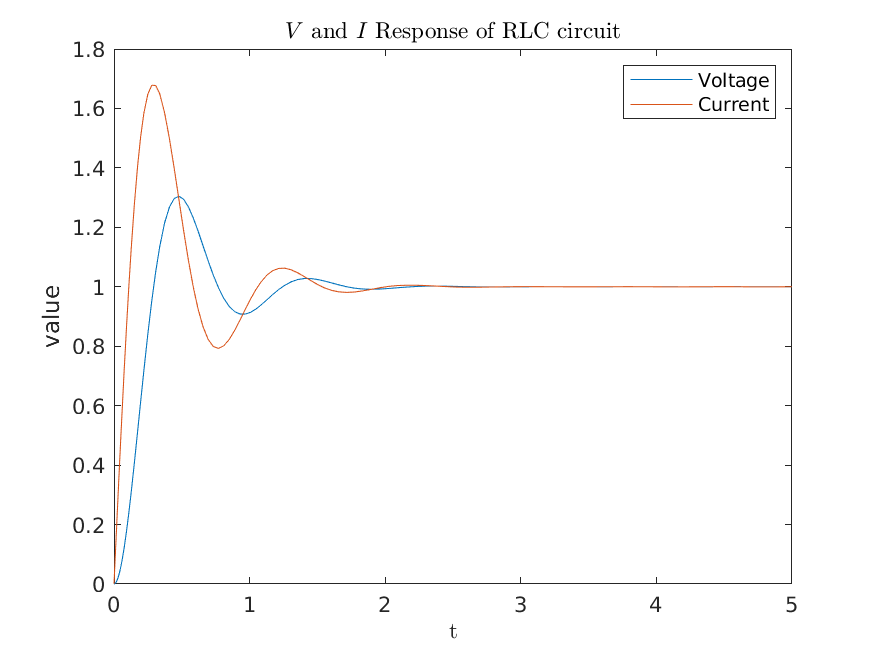
\includegraphics[width = 0.6 \textwidth]{ES155P2_1c_VIresponse.png}
            \caption{Step response of RLC circuit form Figure \ref{fig:RLCcircuit}.}
            \label{fig:VIresponse}
        \end{figure}

        See attached MATLAB code.

    \end{enumerate}

    \item % Problem 2
    \begin{enumerate}
        \item % Part a
        For the control input $u(t) = \begin{bmatrix} v(t) \\ \omega(t) \end{bmatrix}$ and state $z(t) = \begin{bmatrix} x(t) \\ y(t) \\ \theta(t) \end{bmatrix}$, the state space can be written in the form $\dot{z} = f(z, u)$.  As stated, $\dot{\theta}(t) = \omega(t)$, $v_x = v \cos\theta$, and $v_y = v \sin\theta$.  Thus,

        \begin{align}
            \dot{z}(t) &= \begin{bmatrix} \dot{x}(t) \\ \dot{y}(t) \\ \dot{\theta}(t) \end{bmatrix} = \begin{bmatrix} v_x(t) \\ v_y(t) \\ \omega(t) \end{bmatrix} = \begin{bmatrix} v \cos\theta \\ v \sin\theta \\ \omega(t) \end{bmatrix}
        \end{align}

        \item % Part b
        For initial condition $z(0) = \begin{bmatrix} x(0) \\ y(0) \\ \theta(0) \end{bmatrix} = \begin{bmatrix} 0 \\ 0 \\ 0 \end{bmatrix}$ and setting the control input $u(t) = \begin{bmatrix} v(t) \\ \omega(t) \end{bmatrix} =  \begin{bmatrix} c \\ 0 \end{bmatrix}$ for all time $t \ge 0$, the dynamics of the system reduce to a single dimension.  Because $\omega(t) = 0$ for all time $t \ge 0$, $\theta(t) = \theta(0)$, which means $\theta(t) = 0$ for all time $t \ge 0$.  It follows then that, because $y(0) = 0$ and $\theta(0) = 0$, $y(t) = 0$ for all time $t \ge 0$ as well.  Thus, the only state variable that varies with time is $x(t)$.

        As $v(t)$ is fixed at a constant $c$ for all time $t \ge 0$, we can solve for the position by integrating:

        \begin{align}
            x(t) &= \int_0^t v(t) dt + x(0) = ct
        \end{align}

        Thus the solution of the dynamics of this system with these conditions is given by 

        \begin{align}
            z(t) = \begin{bmatrix} x(t) \\ y(t) \\ \theta(t) \end{bmatrix} = \begin{bmatrix} ct \\ 0 \\ 0 \end{bmatrix}
        \end{align}

        \item % Part c
        For initial condition $z(0) = \begin{bmatrix} x(0) \\ y(0) \\ \theta(0) \end{bmatrix} = \begin{bmatrix} 0 \\ -c/b \\ 0 \end{bmatrix}$ and setting the control input $u(t) = \begin{bmatrix} v(t) \\ \omega(t) \end{bmatrix} =  \begin{bmatrix} c \\ b \end{bmatrix}$ for all time $t \ge 0$, we can similarly derive the solution to the dynamics of the system.  Recall from part (a)

        \begin{align}
            \dot{z}(t) &= \begin{bmatrix} \dot{x}(t) \\ \dot{y}(t) \\ \dot{\theta}(t) \end{bmatrix} = \begin{bmatrix} v \cos\theta \\ v \sin\theta \\ \omega(t) \end{bmatrix} \\
            &= \begin{bmatrix} c \cos\theta \\ c \sin\theta \\ b \end{bmatrix}
        \end{align}

        Because $\omega(t) = b$, a constant, for all time $t \ge 0$, $\theta(t)$ is given by

        \begin{align}
            \theta(t) &= \int_0^t \omega(t)dt + \theta(0) = bt
        \end{align}

        we can write

        \begin{align}
            \dot{z}(t) &= \begin{bmatrix} c \cos(bt) \\ c \sin(bt) \\ b \end{bmatrix}
        \end{align}

        To find the solution, guess the answer of the form

        \begin{align}
            z(t) &= \begin{bmatrix} \frac{c}{b} \sin(bt) + C_1 \\ -\frac{c}{b} \cos(bt) + C_2 \\ bt + C_3 \end{bmatrix}
        \end{align}       

        To find the constants, plug in $t = 0$ the initial condition

        \begin{align}
            z(0) = \begin{bmatrix} \frac{c}{b} \sin(b \dot 0) + C_1 \\ -\frac{c}{b} \cos(b \dot 0) + C_2 \\ b \dot 0 + C_3 \end{bmatrix} &= \begin{bmatrix} 0 \\ -c/b \\ 0 \end{bmatrix} \\
            \begin{bmatrix} C_1 \\ -c/b + C_2 \\ C_3 \end{bmatrix} &= \begin{bmatrix} 0 \\ -c/b \\ 0 \end{bmatrix} \\
            \begin{bmatrix} C_1 \\ C_2 \\ C_3 \end{bmatrix} &= \begin{bmatrix} 0 \\ 0 \\ 0 \end{bmatrix}
        \end{align}

        Thus, the solution to the dynamics of the system is given by

        \begin{align}
            z(t) &= \begin{bmatrix} \frac{c}{b} \sin(bt) \\ -\frac{c}{b} \cos(bt) \\ bt \end{bmatrix}
        \end{align} 

        The radius of the position $\sqrt{x^2(t) + y^2(t)}$ is related to the control input:

        \begin{align}
            r &= \sqrt{x^2(t) + y^2(t)} \\
            &= \sqrt{ \left(\frac{c}{b} \right)^2 \sin^2(bt) + \left(-\frac{c}{b} \right)^2 \cos^2(bt)} \\
            &= \frac{c}{b}
        \end{align}

    \end{enumerate}


    \item % Problem 3
    \begin{enumerate}
    	\item % Part a
    	The determinant of matrix $
    	 \begin{bmatrix}
		  a & b \\
		  c & d
		 \end{bmatrix}
		$ is given by $ ad - bc$.

    	\item % Part b
    	The rank of matrix $
    	\begin{bmatrix}
		  1 & 1 \\
		  1 & 2
		 \end{bmatrix}
		 $ can be found by reducing the matrix to row echelon form, then counting the number of non-zero rows.  In this case, the matrix reduces to the identity matrix, so the rank is just the number of rows, 2.

    	\item % Part c
    	In this case, the matrix $
    	\begin{bmatrix}
		  1 & 1 \\
		  0 & 0
		 \end{bmatrix}
    	$is already in reduced row echelon form and the there is only one non-zero row, as well as only one linearly independent column, so the rank is 1.

    	\item % Part d
    	The matrix $
    	\begin{bmatrix}
		  1 & 1 & 0 \\
		  1 & 1 & 1
		 \end{bmatrix}
    	$reduces to$
    	\begin{bmatrix}
		  1 & 1 & 0 \\
		  0 & 0 & 1
		 \end{bmatrix}
		 $.  There are two non-zero rows, so the row rank is 2.

    	\item % Part e
    	The matrix $
    	\begin{bmatrix}
		  1 & 1 & 0 \\
		  1 & 1 & 1
		 \end{bmatrix}
    	$reduces to$
    	\begin{bmatrix}
		  1 & 1 & 0 \\
		  0 & 0 & 1
		 \end{bmatrix}
		 $ (same as part d).  There are only two linearly independent columns, so the column rank is 2.

    	\item % Part f
    	The matrix $
    	\begin{bmatrix}
		  1 & 1 \\
		  1 & 1 \\
		  0 & 1
		 \end{bmatrix}
    	$reduces to$
    	\begin{bmatrix}
		  1 & 0 \\
		  0 & 1 \\
		  0 & 0
		 \end{bmatrix}
		 $.  Note that this matrix was the transpose of the one given in parts d and e.  As there are two non-zero rows, the rank of the matrix is 2.

    	\item % Part g
    	The matrix $
    	\begin{bmatrix}
		  1 & 1 \\
		  1 & 1 \\
		  0 & 1
		 \end{bmatrix}
    	$reduces to$
    	\begin{bmatrix}
		  1 & 0 \\
		  0 & 1 \\
		  0 & 0
		 \end{bmatrix}
		 $.  There are two linearly-independent columns, so the again is 2.

    	\item % Part h
    	The last four parts all have the same rank.  This suggests that the row and column ranks of a matrix are the same, and the rank of a matrix and its transpose are the same as well, because the rows and columns of a matrix's transpose are the columns and rows of the original matrix, and the column and row ranks are equivalent.

    \end{enumerate}

\end{enumerate}
\end{document}


